\chapter{Acerca de DYNAMITE} \label{chap:dynamite}

DYNAMITE es una herramienta de software que fue desarrollada por el autor de la presente monografía como una forma didáctica de apoyo para el trabajo con sistemas dinámicos planos, los continuos en particular y que fue utilizada para generar todos los diagramas de fase en este documento.

La inspiración para DYNAMITE se encuentra en Phaser \cite{phaser}, software que acompaña al libro ``Dynamics and Bifurcations'' \cite{dynandbif} de J. Hale y H. Ko\c{c}ak o puede adquirirse también a través del sitio web.

Phaser ha evolucionado durante años hasta convertirse en un completo paquete de software para la simulación de todo tipo de sistemas dinámicos y no se encuentra limitado únicamente a sistemas planos. En estas condiciones DYNAMITE no apunta a replicar la funcionalidad que se encuentra ya en Phaser, sino más bien proveer una base sólida sobre la cual pudiera llegar a construirse una aplicación comparable, pero a través de una filosofía muy diferente a la de los autores de Phaser: la del software libre.

En consecuencia, DYNAMITE no tiene costo alguno y su código fuente se encuentra disponible en línea \cite{dynamite} para ser reutilizado o modificado por quien así lo desee sin restricción alguna.

Aún cuando el autor considera que el alto costo de software especializado como Phaser está muchas veces bien justificado, en la mayoría de las ocasiones impide que sea adquirido por estudiantes universitarios, quienes se esperaría fueran sus principales usuarios.
Aunque es una visión ambiciosa, DYNAMITE pretende ayudar a cerrar esta brecha entre software comercial y libre al menos en el área de los sistemas dinámicos, donde en la actualidad hay muy pocas posibilidades para quienes no cuenten con suficientes recursos económicos o el conocimiento computacional para hacer sus propias rutinas de software.

En particular, en cuanto a software gratuito, la mayoría del código disponible es de carácter académico \cite{chaospython,chaosatmaryland,stonydynamics,cornelldynamics} y no se refiere nunca a una aplicación destinada a usuarios finales, o requiere para su ejecución de entornos de carácter pago como MATLAB o Mathematica.

\begin{figure}[!ht] \centering
	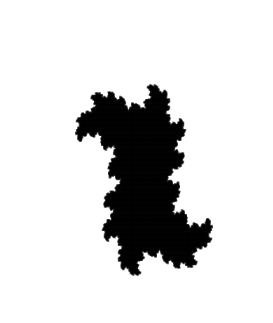
\includegraphics[scale=0.7]{figures/juliaset.png}
	\caption{$\clubsuit$ Conjunto de Julia para $c = 0.835 - 0.2321i$ generado con DYNAMITE.}
	\label{fig:dynamite}
\end{figure}

\section{Resumen de características}

A continuación hacemos una lista, no extensiva, de las principales características disponibles al momento en DYNAMITE.

\begin{itemize}
	\item DYNAMITE es software libre: su distribución y modificación está permitida sin restricciones.
	\item Debido a su diseño, basado en el lenguaje de programación Python \cite{python} y la librería multiplataforma Qt \cite{libqt}, DYNAMITE puede ser ejecutado -sin modificación- en cualquier sistema Mac OS X, Linux o Windows.
	\item DYNAMITE tiene una interfaz moderna y produce gráficas vectoriales con antialiasing \cite{pcmagantialiasing} de nivel apto para publicación que pueden ser personalizadas en cuanto a tipo de líneas, color, etc.
	\item DYNAMITE soporta una amplia gama de funciones estándar como lo son funciones exponenciales, trigonométricas, etc. que pueden ser utilizadas en las expresiones matemáticas que se ingresan en la aplicación.
	\item En este momento, cualquiera de los siguientes gráficos puede ser generado por DYNAMITE:
		\begin{itemize}
			\item Campos de pendientes asociadas a un sistema dinámico.
			\item Órbitas arbitrarias de un sistema dinámico plano continuo para constituir un retrato de fase.
			\item Conjuntos de Julia \cites{complexdynamics,milnorcomplex} asociados a sistemas dinámicos complejos discretos obtenidos por iteración a partir del polinomio cuadrático $f_c(z) = z^2 + c$, $z \in \C$.
		\end{itemize}
	\item DYNAMITE permite utilizar dos tipos de integradores diferentes para aproximar numéricamente las soluciones de los sistemas de ecuaciones diferenciales involucrados: un método Runge-Kutta combinado de órdenes 4 y 5 \cites[p.~518]{analisisnumerico}{fehlberg} y el método ``backward Euler'' \cites[p.~584]{analisisnumerico}{butcher}. De esta manera DYNAMITE  trata con ecuaciones ``stiff'' \cites{stiff}[p.~583]{analisisnumerico} y ``non-stiff'' \cite{nonstiff}.
\end{itemize}

\section{Información de descarga y licencia}

La última versión de DYNAMITE, así como su código fuente, se encuentran disponibles públicamente en el sitio web \url{https://github.com/jorgeatorres/dynamite}.

El código está distribuído bajo la licencia WTFPL \cite{wtfpl}. Queda como ejercicio al lector revisar las condiciones (¡así como el significado de las siglas!) de la licencia en la referencia. El creador de la licencia, Sam Hocevar, la define así: ``A very permissive license for software and other scientific or artistic works that offers a great degree of freedom''.